% Generated by Sphinx.
\documentclass[letterpaper,10pt,english]{manual}
\usepackage[utf8]{inputenc}
\usepackage[T1]{fontenc}
\usepackage{babel}
\usepackage{times}
\usepackage[Bjarne]{fncychap}
\usepackage{longtable}
\usepackage{sphinx}


\title{Cloud Files Developer Guide Documentation}
\date{August 12, 2009}
\release{1.1.0}
\author{Eric "EJ" Johnson}
\newcommand{\sphinxlogo}{}
\renewcommand{\releasename}{Release}
\makeindex

\newcommand\PYGZat{@}
\newcommand\PYGZlb{[}
\newcommand\PYGZrb{]}
\newcommand\PYGaz[1]{\textcolor[rgb]{0.00,0.63,0.00}{#1}}
\newcommand\PYGax[1]{\textcolor[rgb]{0.84,0.33,0.22}{\textbf{#1}}}
\newcommand\PYGay[1]{\textcolor[rgb]{0.00,0.44,0.13}{\textbf{#1}}}
\newcommand\PYGar[1]{\textcolor[rgb]{0.73,0.38,0.84}{#1}}
\newcommand\PYGas[1]{\textcolor[rgb]{0.25,0.44,0.63}{\textit{#1}}}
\newcommand\PYGap[1]{\textcolor[rgb]{0.78,0.36,0.04}{#1}}
\newcommand\PYGaq[1]{\textcolor[rgb]{0.38,0.68,0.84}{#1}}
\newcommand\PYGav[1]{\textcolor[rgb]{0.00,0.44,0.13}{\textbf{#1}}}
\newcommand\PYGaw[1]{\textcolor[rgb]{0.13,0.50,0.31}{#1}}
\newcommand\PYGat[1]{\textcolor[rgb]{0.32,0.47,0.09}{#1}}
\newcommand\PYGau[1]{\textcolor[rgb]{0.13,0.50,0.31}{#1}}
\newcommand\PYGaj[1]{\textcolor[rgb]{0.00,0.44,0.13}{#1}}
\newcommand\PYGak[1]{\textcolor[rgb]{0.14,0.33,0.53}{#1}}
\newcommand\PYGah[1]{\textcolor[rgb]{0.00,0.13,0.44}{\textbf{#1}}}
\newcommand\PYGai[1]{\textcolor[rgb]{0.73,0.38,0.84}{#1}}
\newcommand\PYGan[1]{\textcolor[rgb]{0.00,0.44,0.13}{\textbf{#1}}}
\newcommand\PYGao[1]{\textcolor[rgb]{0.25,0.44,0.63}{\textbf{#1}}}
\newcommand\PYGal[1]{\colorbox[rgb]{1.00,0.94,0.94}{\textcolor[rgb]{0.25,0.50,0.56}{#1}}}
\newcommand\PYGam[1]{\textbf{#1}}
\newcommand\PYGab[1]{\textit{#1}}
\newcommand\PYGac[1]{\textcolor[rgb]{0.25,0.44,0.63}{#1}}
\newcommand\PYGaa[1]{\textcolor[rgb]{0.19,0.19,0.19}{#1}}
\newcommand\PYGaf[1]{\textcolor[rgb]{0.25,0.50,0.56}{\textit{#1}}}
\newcommand\PYGag[1]{\textcolor[rgb]{0.13,0.50,0.31}{#1}}
\newcommand\PYGad[1]{\textcolor[rgb]{0.25,0.44,0.63}{#1}}
\newcommand\PYGae[1]{\textcolor[rgb]{0.13,0.50,0.31}{#1}}
\newcommand\PYGaZ[1]{\textcolor[rgb]{0.02,0.16,0.45}{\textbf{#1}}}
\newcommand\PYGbf[1]{\textcolor[rgb]{0.40,0.40,0.40}{#1}}
\newcommand\PYGaX[1]{\textcolor[rgb]{0.00,0.44,0.13}{#1}}
\newcommand\PYGaY[1]{\textcolor[rgb]{0.25,0.44,0.63}{#1}}
\newcommand\PYGbc[1]{\textcolor[rgb]{0.00,0.44,0.13}{\textbf{#1}}}
\newcommand\PYGbb[1]{\textcolor[rgb]{0.13,0.50,0.31}{#1}}
\newcommand\PYGba[1]{\textcolor[rgb]{0.00,0.00,0.50}{\textbf{#1}}}
\newcommand\PYGaR[1]{\textcolor[rgb]{0.73,0.38,0.84}{#1}}
\newcommand\PYGaS[1]{\textcolor[rgb]{0.25,0.50,0.56}{\textit{#1}}}
\newcommand\PYGaP[1]{\textcolor[rgb]{0.25,0.44,0.63}{#1}}
\newcommand\PYGaQ[1]{\textcolor[rgb]{0.13,0.50,0.31}{#1}}
\newcommand\PYGaV[1]{\textcolor[rgb]{0.05,0.52,0.71}{\textbf{#1}}}
\newcommand\PYGaW[1]{\textcolor[rgb]{0.25,0.44,0.63}{#1}}
\newcommand\PYGaT[1]{\textcolor[rgb]{0.50,0.00,0.50}{\textbf{#1}}}
\newcommand\PYGaU[1]{\textcolor[rgb]{0.00,0.44,0.13}{#1}}
\newcommand\PYGaJ[1]{\textcolor[rgb]{0.25,0.44,0.63}{#1}}
\newcommand\PYGaK[1]{\textcolor[rgb]{0.02,0.16,0.49}{#1}}
\newcommand\PYGaH[1]{\fcolorbox[rgb]{1.00,0.00,0.00}{1,1,1}{#1}}
\newcommand\PYGaI[1]{\textcolor[rgb]{0.56,0.13,0.00}{#1}}
\newcommand\PYGaN[1]{\textcolor[rgb]{0.05,0.52,0.71}{\textbf{#1}}}
\newcommand\PYGaO[1]{\textcolor[rgb]{0.78,0.36,0.04}{\textbf{#1}}}
\newcommand\PYGaL[1]{\textcolor[rgb]{0.73,0.73,0.73}{#1}}
\newcommand\PYGaM[1]{\textcolor[rgb]{0.00,0.44,0.13}{#1}}
\newcommand\PYGaB[1]{\textcolor[rgb]{0.00,0.25,0.82}{#1}}
\newcommand\PYGaC[1]{\textcolor[rgb]{0.33,0.33,0.33}{\textbf{#1}}}
\newcommand\PYGaA[1]{\textcolor[rgb]{0.00,0.44,0.13}{#1}}
\newcommand\PYGaF[1]{\textcolor[rgb]{1.00,0.00,0.00}{#1}}
\newcommand\PYGaG[1]{\textcolor[rgb]{0.73,0.38,0.84}{#1}}
\newcommand\PYGaD[1]{\textcolor[rgb]{0.25,0.50,0.56}{\textit{#1}}}
\newcommand\PYGaE[1]{\textcolor[rgb]{0.63,0.00,0.00}{#1}}
\newcommand\PYGbg[1]{\textcolor[rgb]{0.44,0.63,0.82}{\textit{#1}}}
\newcommand\PYGbe[1]{\textcolor[rgb]{0.25,0.44,0.63}{#1}}
\newcommand\PYGbd[1]{\textcolor[rgb]{0.00,0.44,0.13}{\textbf{#1}}}
\newcommand\PYGbh[1]{\textcolor[rgb]{0.00,0.44,0.13}{\textbf{#1}}}
\begin{document}

\maketitle
\tableofcontents




\chapter{Overview}

The Rackspace Cloud Files™ is an affordable, redundant, scalable, and
dynamic storage service offering.  The core storage system is designed to
provide a safe, secure, automatically re-sizing and network accessible way
to store data.  You can store an unlimited quantity of files and each file
can be as large as 5 gigabytes. Users can store as much as they want and
pay only for storage space they actually use.

Additionally, Cloud Files provides a simple yet powerful way to publish
and distribute content behind the industry leading Limelight Networks'
Content Distribution Network. Cloud Files users get access to this
network automatically without having to worry about contracts, additional
costs, or technical hurdles.

Cloud Files allows users to store/retrieve files and CDN-enable content
via a simple Web Service (ReST: Representational State Transfer)
interface. There are also language-specific API’s that utilize the ReST
API but make it much easier for developers to integrate into their
applications.

For more details on the Cloud Files service please refer to
\href{http://www.rackspacecloud.com/cloud\_hosting\_products/files}{http://www.rackspacecloud.com/cloud\_hosting\_products/files}


\chapter{Intended Audience}

This document is intended for software developers who have chosen to use
Cloud Files. It fully documents the ReST application programming interface
(API) that allows developers to interact with the storage and CDN
components of the Cloud Files system.
\begin{quote}

Prerequisites: Familiarity with HTTP, RFC 2616
\end{quote}

Rackspace also provides company supported language-specific API’s in
several popular programming languages.  The current list of supported
API’s is C\#/.NET, Java, PHP, Python, and Ruby.  These API’s utilize the
ReST API and are provided to help developers rapidly integrate Cloud Files
support into their applications without needing to write at the ReST
interface.  Each API includes its own documentation in its “native”
format.  For example, the Java API includes JavaDocs and the C\#/.NET API
includes a CHM file.

System administrators and other users who are interested in the storage
and CDN benefits of Cloud Files, should consider using the File Manager
interface within the Rackspace Cloud Control Panel or third party tools
like \href{http://www.fireuploader.com/}{Fireuploader}, \href{http://www.cyberduck.ch/}{Cyberduck}, and \emph{Cloud Files Manager\_}.  The control
panel provides an easy to use web-based interface for uploading/downloading
content to Cloud Files.


\chapter{Concepts}

Cloud Files is not a “file system” in the traditional sense. You will not
be able to \textbf{map} or \textbf{mount} virtual disk drives like you can with
other forms of storage such as a SAN or NAS. Since Cloud Files is a
different way of thinking when it comes to storage so you should take a
few moments to review the key concepts listed below.


\section{Accounts}

The Cloud Files system is designed to be used by many different customers.
Your user account is your portion of the Cloud Files system. A user must
identify themselves with their Rackspace Cloud username and API Access Key
and once authenticated, that user has full read/write access to the files
stored under that user account. Please visit \href{http://www.rackspacecloud.com}{http://www.rackspacecloud.com}
to obtain a Cloud Files account and enable your API Access Key.


\section{Authentication}

The language and ReST API's below describe how to authenticate against the
Authentication service to receive Cloud Files connection parameters and an
“authentication token”.  The token must be passed in for all subsequent
Container/Object operations.

\begin{notice}{note}{Note:}
The language-specific API's handle authentication, token passing,
and HTTPS request/response communication.
\end{notice}


\section{Permissions}

There are no permissions or access-controls around Containers or Objects
in Cloud Files.  Each user has their own storage account and has full
access to that account. Users must authenticate with their credentials as
described above, but once authenticated they can create/delete Containers
and Objects within that Account.  The only way a user can access the
content from another Account is if they share their Username/API Access
Key or a session token.


\section{Containers}

A Container is a “storage compartment” for your data and provides a way
for you to organize your data. You can think of a Container as a folder
in Windows® or a directory in UNIX®. The primary difference between a
Container and these other “file system” concepts is that Containers cannot
be nested. You can, however, create an unlimited number of Containers
within your account.  Data must be stored in a Container so you must have
at least one Container defined in your account prior to uploading data.

The only restrictions on Container names is that they cannot contain a
forward slash, “/” character must be less than 256 bytes in length.
Please note that the length restriction applies to the name after it has
been URL encoded.  For example, a Container name of “Course Docs” would be
URL encoded as “Course\%20Docs” and therefore be 13 bytes in length rather
than the expected 11.


\section{Objects}

An “Object” is the basic storage entity and any optional metadata that
represents the “files” you store in the Cloud Files system. When you
upload data to Cloud Files the data is stored as-is (no compression or
encryption) and consists of a location (Container), the Object's name,
and any metadata consisting of key/value pairs. For instance, you may
chose to store a backup of your digital photos and organize them into
albums.  For example, each Object could be tagged with metadata such as
“Album : Caribbean Cruise” or “Album : Aspen Ski Trip”.

The only restriction on Object names is that they must be less than 1024
bytes in length after URL encoding.  For example, an Object name of
“C++final(v2).txt” should be URL encoded as “C\%2B\%2Bfinal\%28v2\%29.txt”
and therefore be 24 bytes in length rather than the expected 16.

The maximum allowable size for a storage Object is 5 gigabytes and the
minimum is zero bytes.  For metadata, you should not exceed 90 individual
key/value pairs for any one Object and the and the total byte length of
all key/value pairs should not exceed 4KB (4096 bytes).


\section{Operations}

Operations are the actions you perform within your Account. Creating or
deleting Containers, uploading or downloading Objects, etc. The full list
of operations is documented under the ReST API section. Operations may be
performed via the ReST web service API or a language-specific API
(currently we support Python, PHP, Java, Ruby, and C\#/.NET).

\begin{notice}{note}{Note:}
All operations must include a valid authorization token.
\end{notice}


\section{CDN-enabled Containers}

To publish data that is to be served by Limelight Networks' Content
Distribution Network (CDN), Containers which house the data must be
“CDN-enabled”.  When a Container is CDN-enabled any files will be
publicly accessible and not require an authentication token for read
access.  Uploading content into a CDN-enabled Container is a secure
operation and will require a valid authentication token.

Each CDN-enabled Container has a unique Uniform Resource Locator (URL)
that can be combined with its Object names and openly distributed in web
pages, emails, or other applications.

For example, a CDN-enabled Container named \emph{photos} might be referenced as
\href{http://c0010171.cdn.cloudfiles.rackspacecloud.com}{http://c0010171.cdn.cloudfiles.rackspacecloud.com}.  If that Container
houses a screenshot called \emph{wow1.jpg}, then that image can be served by
Limelight Networks' CDN with the full URL of
\href{http://c0010171.cdn.cloudfiles.rackspacecloud.com/wow1.jpg}{http://c0010171.cdn.cloudfiles.rackspacecloud.com/wow1.jpg}.  This URL can
be embedded in HTML pages, email messages, blog posts, etc.  When that URL
is accessed, a copy of that image is fetched from the Cloud Files storage
system and cached in Limelight Networks' CDN and served from there for
all subsequent requests for a configurable cache timeout (TTL) value.
Setting the TTL of a CDN-enabled Container translates to setting the
\code{Expires} and \code{Cache-Control} HTTP headers.

Containers tracked in the CDN management service are completely separate
and distinct from the Containers defined in the storage service.  It
is possibly for a Container to be CDN-enabled even if it doesn't exist
in the storage system.  Users may want the ability to pre-generate
CDN URL's before actually uploading content and this separation gives
them that ability.

However, for the content to be served from the CDN, the Container names
\textbf{MUST} match in both the CDN management service and the storage service.
For example, you could CDN-enable a Container called \emph{images} and be
assigned the CDN URL, but you also need to create a Container called
\emph{images} in the storage service.

For more details on the CDN operations refer to “Content Delivery Networks
with Cloud Files”


\chapter{Language-specific API's}

A set of supported API's in several popular languages are available to
help put Cloud Files in the hands of developers.  These API's provide a
layer of abstraction on top of the base ReST API allowing programmers to
work with a Container and Object model instead of working directly with
HTTP requests and responses.   These API's are free (as in beer and as in
speech) to download, use, and modify.  They are all licensed under the
MIT license as described in the COPYING file packaged with each API.  If
you do make any improvements to an API, you are encouraged (but not
required) to submit those changes back to us.

The API's are hosted at \href{http://github.com/rackspace}{http://github.com/rackspace}.  Feel free to
coordinate your changes through github or if you prefer, send
your changes to \href{mailto:cloudfiles@rackspacecloud.com}{cloudfiles@rackspacecloud.com}.  Just make sure to
indicate which language and version you modified and send us a unified
diff.

Each API includes its own documentation (either HTML, PDF, or CHM).
They also include code snippets and examples to help you get started.
The currently supported API's for Cloud Files are:
\begin{itemize}
\item {} 
PHP (requires 5.x and the modules: cURL, FileInfo, mbstring)

\item {} 
Python (requires 2.4 or newer)

\item {} 
Java (requires JRE v1.5 or newer)

\item {} 
C\#/.NET (requires .NET Framework v3.5)

\item {} 
Ruby (requires 1.8 or newer and mime-tools module)

\end{itemize}

There are no other supported language-specific API's at this time.  You
are welcome to create your own language API's and we will help answer any
questions during development, host your code if you like, and give you
full credit for your work.


\chapter{ReST API's}

The underlying API for Cloud Files is implemented as a set of ReSTful
web services (Representational State Transfer). All Authentication and
Container/Object operations can be performed with standard HTTP calls.
See the \href{http://en.wikipedia.org/wiki/Representational\_State\_Transfer}{Wikipedia article} for more information about ReST.

The following constraints apply to the ReST API's HTTP requests:
\begin{itemize}
\item {} 
Maximum number of HTTP headers per request: 90

\item {} 
Maximum length of all HTTP headers: 4096 bytes

\item {} 
Maximum length per HTTP request line: 8192 bytes

\item {} 
Maximum length of HTTP request: 5 gigabytes

\item {} 
Maximum length of Container name: 256 bytes

\item {} 
Maximum length of Object name: 1024 bytes

\end{itemize}

Container and Object names should be properly URL encoded prior
to interacting with the ReST interface (the language API's handle
URL encoding/decoding).  The length restrictions should be checked
against the URL encoded string.

Each ReST request against the Cloud Files system requires the inclusion of
a specific “authorization token” HTTP header defined as \code{X-Auth-Token}.
Clients obtain this token, along with the Cloud Files URI's, by first
using the Authentication service and supplying a valid Username and API
Access Key.

There are actually two different sets of ReST services that make up the
full Cloud Files product.  The first ReST service identified with
\code{X-Storage-Url} is used for managing the data stored in the system.
Example operations are creating Containers and uploading Objects.  The
second ReST service is for managing the CDN feature of Cloud Files and is
identified by \code{X-CDN-Management-Url}.

In the following sections, each HTTP method will be documented and which
service the call should be made against.  For example, a \code{PUT} request
against \code{X-Storage-Url} can be used to create a Container or upload an
Object.  A \code{PUT} request against the \code{X-CDN-Management-Url} is used
to CDN-enable a Container.

The language-specific API's mask this system separation from the
programmer.  They simply create a Container and mark it “public” and it
handles calling out to the appropriate back-end services using the
appropriate ReST API.

\begin{notice}{note}{Note:}
All requests to authenticate and operate against Cloud Files are
performed using SSL over HTTP (HTTPS) on TCP port 443.
\end{notice}

The following diagram illustrates the various system interfaces and the
ease with which content can be distributed over the CDN.  Authenticate,
create a Container, upload Objects, mark the Container as \emph{public} and
begin serving that content from Limelight Networks' powerful CDN.

{\hfill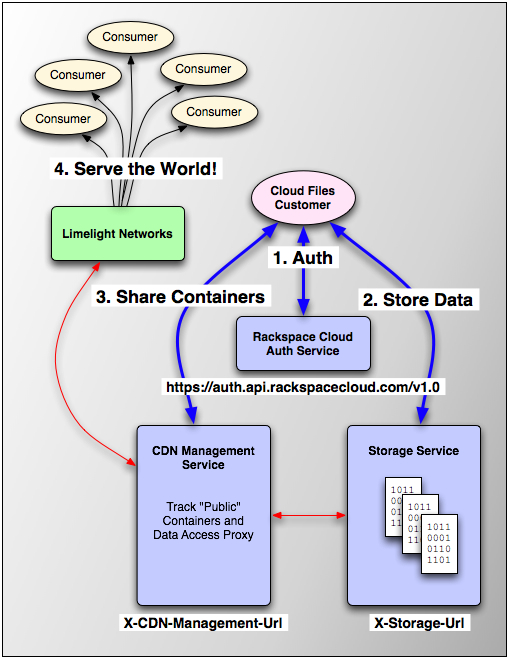
\includegraphics{cf-systems.jpg}\hfill}


\section{Authentication}

In order to use the Cloud Files storage system, you must first have a
valid username and API Access Key. Include these parameters as HTTP
headers in the authentication request illustrated below.


\subsection{Request}

Client authentication is provided via a ReST interface using the \code{GET}
method, with `auth' supplied as the path. Additionally, two headers are
required, \code{X-Auth-User} and \code{X-Auth-Key} with values for the username
and API Access Key respectively.

Sample request:

\begin{Verbatim}[commandchars=@\[\]]
GET /v1.0 HTTP/1.1
Host: auth.api.rackspacecloud.com
X-Auth-User: jdoe
X-Auth-Key: a86850deb2742ec3cb41518e26aa2d89
\end{Verbatim}


\subsection{Response}

When authentication is successful, an HTTP status 204 (No Content) is
returned with three headers, \code{X-Storage-Url}, \code{X-CDN-Management-Url},
and \code{X-Auth-Token}. An HTTP status of 401 (Unauthorized) is returned
upon authentication failure. All subsequent Container/Object operations
against Cloud Files should be made against the URI specified in
\code{X-Storage-Url} or \code{X-CDN-Management-Url} and must include the
\code{X-Auth-Token} header.

Sample response:

\begin{Verbatim}[commandchars=@\[\]]
HTTP/1.1 204 No Content
Date: Mon, 12 Nov 2007 15:32:21 GMT
Server: Apache
X-Storage-Url: https://storage.clouddrive.com/v1/CF@_xer7@_34
X-CDN-Management-Url: https://cdn.clouddrive.com/v1/CF@_xer7@_34
X-Auth-Token: eaaafd18-0fed-4b3a-81b4-663c99ec1cbb
Content-Length: 0
Content-Type: text/plain; charset=UTF-8
\end{Verbatim}

The \code{X-Storage-Url} and \code{X-CDN-Management-Url} will need to be parsed
and used in the connection and request line of all subsequent requests
against Cloud Files. In the example response above, users connecting to
Cloud Files would send most Container/Object requests with a Host header
of \emph{storage.clouddrive.com} and the request line's version and account as
\code{/v1/CF\_xer7\_34}.  To CDN-enable Containers or adjust CDN
attributes, ReST requests should be sent to \emph{cdn.clouddrive.com}. Note
that authentication tokens are valid for a 24 hour period.


\section{Storage Services}

The following section describes the ReST API for interacting with the
storage component of Cloud Files.  All requests will be directed to the
host and URL described in the \code{X-Storage-Url} HTTP header obtained
during successful authentication.

The following are some pointers for the use of the Storage services:
\begin{itemize}
\item {} 
Container names cannot exceed 256 bytes and cannot contain a `/'
character

\item {} 
Object names cannot exceed 1024 bytes and have no character
restrictions

\item {} 
Object and Container names must be URL-encoded

\end{itemize}


\subsection{Storage Account Services}

The following operations can be performed at the account level of the URI.
For example, the URI for the requests below will end with the Cloud Files
account string:

\begin{Verbatim}[commandchars=@\[\]]
METHOD /v1/@textless[]account@textgreater[] HTTP/1.1
\end{Verbatim}


\subsubsection{GET}

\code{GET} operations against the \code{X-Storage-Url} for an account are
performed to retrieve a list of existing storage Containers ordered by
name.  The following list describes the optional query parameters that
are supported with this request.
\begin{itemize}
\item {} 
\textbf{limit} - For an integer value N, limits the number of results to
at most N values.

\item {} 
\textbf{marker} - Given a string value X, return Object names greater in
value than the specified marker.

\item {} 
\textbf{format} - Specify either \emph{json} or \emph{xml} to return the respective
serialized response.

\end{itemize}

At this time, a “prefix” query parameter is not supported at the Account
level.


\paragraph{Request}

The list of storage Containers is returned in the response body, one
Container name per line.

Sample request:

\begin{Verbatim}[commandchars=@\[\]]
GET /@textless[]api version@textgreater[]/@textless[]account@textgreater[] HTTP/1.1
Host: storage.clouddrive.com
X-Auth-Token: eaaafd18-0fed-4b3a-81b4-663c99ec1cbb
\end{Verbatim}


\paragraph{Response}

A list of containers is returned in the response body, one container per
line. A 204 (No Content) HTTP return code will be passed back if the
account has no containers.

Sample response:

\begin{Verbatim}[commandchars=@\[\]]
HTTP/1.1 200 Ok
Date: Thu, 07 Jun 2007 18:57:07 GMT
Server: Apache
Content-Type: text/plain; charset=UTF-8
Content-Length: 32

images
movies
documents
backups
\end{Verbatim}


\paragraph{Serialized List Output}

If a \code{format=xml} or \code{format=json} argument is appended to the storage
account URL, the service will serve extended container information
serialized in the chosen format.  The sample responses below are formatted
for readability.

Sample JSON format request:

\begin{Verbatim}[commandchars=@\[\]]
GET /@textless[]api version@textgreater[]/@textless[]account@textgreater[]?format=json HTTP/1.1
Host: storage.clouddrive.com
Content-Length: 0
X-Storage-Token: 182f9c0af0e828cfe3281767d29d19f4
\end{Verbatim}

Sample JSON response:

\begin{Verbatim}[commandchars=@\[\]]
HTTP/1.1 200 OK
Date: Tue, 25 Nov 2008 19:39:13 GMT
Server: Apache
Content-Type: application/json; charset=utf-8

@PYGZlb[]
  {"name":"test@_container@_1", "count":2, "bytes":78},
  {"name":"test@_container@_2", "count":1, "bytes":17},
@PYGZrb[]
\end{Verbatim}

Sample XML format request:

\begin{Verbatim}[commandchars=@\[\]]
GET /@textless[]api version@textgreater[]/@textless[]account@textgreater[]?format=xml HTTP/1.1
Host: storage.clouddrive.com
Content-Length: 0
X-Storage-Token: 182f9c0af0e828cfe3281767d29d19f4
\end{Verbatim}

Sample XML response:

\begin{Verbatim}[commandchars=@\[\]]
HTTP/1.1 200 OK
Date: Tue, 25 Nov 2008 19:42:35 GMT
Server: Apache
Content-Type: application/xml; charset=utf-8

@textless[]?xml version="1.0" encoding="UTF-8"?@textgreater[]
@textless[]account name="MichaelBarton"@textgreater[]
  @textless[]container@textgreater[]
    @textless[]name@textgreater[]test@_container@_1@textless[]/name@textgreater[]
    @textless[]count@textgreater[]2@textless[]/count@textgreater[]
    @textless[]bytes@textgreater[]78@textless[]/bytes@textgreater[]
  @textless[]/container@textgreater[]
  @textless[]container@textgreater[]
    @textless[]name@textgreater[]test@_container@_2@textless[]/name@textgreater[]
    @textless[]count@textgreater[]1@textless[]/count@textgreater[]
    @textless[]bytes@textgreater[]17@textless[]/bytes@textgreater[]
  @textless[]/container@textgreater[]
@textless[]/account@textgreater[]
\end{Verbatim}


\paragraph{Large Container Lists}

The system will return a maximum of 10,000 Container names per request.
To retrieve subsequent container names, another request must be made with
a `marker' parameter. The marker indicates where the last list left off
and the system will return container names greater than this marker, up to
10,000 again.  Note that the ‘marker’ value should be URL encoded prior to
sending the HTTP request.

If 10,000 is larger than desired, a `limit' parameter may be given.

If the number of container names returned equals the limit given (or
10,000 if no limit is given), it can be assumed there are more container
names to be listed. If the container name list is exactly divisible by the
limit, the last request will simply have no content.

For an example, let's use a listing of five container names:

\begin{Verbatim}[commandchars=@\[\]]
apples
bananas
kiwis
oranges
pears
\end{Verbatim}

We'll use a limit of 2 to show how things work:

\begin{Verbatim}[commandchars=@\[\]]
GET /@textless[]api version@textgreater[]/@textless[]account@textgreater[]?limit=2
Host: storage.clouddrive.com
X-Auth-Token: eaaafd18-0fed-4b3a-81b4-663c99ec1cbb

apples
bananas
\end{Verbatim}

Since we received 2 items back, we can assume there are more container
names to list; so we make another request with a marker of the last item
returned:

\begin{Verbatim}[commandchars=@\[\]]
GET /@textless[]api version@textgreater[]/@textless[]account@textgreater[]?limit=2@&marker=bananas
Host: storage.clouddrive.com
X-Auth-Token: eaaafd18-0fed-4b3a-81b4-663c99ec1cbb

kiwis
oranges
\end{Verbatim}

Again we have 2 items returned, there may be more:

\begin{Verbatim}[commandchars=@\[\]]
GET /@textless[]api version@textgreater[]/@textless[]account@textgreater[]?limit=2@&marker=oranges
Host: storage.clouddrive.com
X-Auth-Token: eaaafd18-0fed-4b3a-81b4-663c99ec1cbb

pears
\end{Verbatim}

Now we received less than the limit number of container names; so we have
the complete list.


\subsubsection{HEAD}

\code{HEAD} operations against an account are performed to retrieve the
number of Containers and the total bytes stored in Cloud Files for the
account. This information is returned in two custom headers,
\code{X-Account-Container-Count} and \code{X-Account-Bytes-Used}.


\paragraph{Request}

Determine the number of Containers within the account and the total bytes
stored.  Since the storage system is designed to store large amounts of
data, care should be taken when representing the total bytes response as
an “integer”; when possible, convert it to a 64-bit unsigned integer if
your platform supports that primitive type.

Sample request:

\begin{Verbatim}[commandchars=@\[\]]
HEAD /@textless[]api version@textgreater[]/@textless[]account@textgreater[] HTTP/1.1
Host: storage.clouddrive.com
X-Auth-Token: eaaafd18-0fed-4b3a-81b4-663c99ec1cbb
\end{Verbatim}


\paragraph{Response}

The HTTP return code will be 204 (No Content) if the request succeeds.
A 401 (Unauthorized) will be returned for an invalid account or access
key.

Sample response:

\begin{Verbatim}[commandchars=@\[\]]
HTTP/1.1 204 No Content
Date: Thu, 07 Jun 2007 18:57:07 GMT
Server: Apache
X-Account-Container-Count: 3
X-Account-Total-Bytes-Used: 323479
\end{Verbatim}


\subsection{Storage Container Services}

This section documents the ReST operations that can be performed on
Containers. All operations are valid HTTP request methods and will
resemble this format:

\begin{Verbatim}[commandchars=@\[\]]
METHOD /v1/@textless[]account@textgreater[]/@textless[]container@textgreater[] HTTP/1.1
\end{Verbatim}


\subsubsection{HEAD}

\code{HEAD} operations against a storage Container are used to determine the
number of Objects, and the total bytes of all Objects stored in the
Container.


\paragraph{Request}

Determine the number of Objects and total stored bytes within the
Container.  Since the storage system is designed to store large amounts
of data, care should be taken when representing the total bytes response
as an “integer”; when possible, convert it to a 64-bit unsigned integer
if your platform supports that primitive type.

Sample request:

\begin{Verbatim}[commandchars=@\[\]]
HEAD /@textless[]api version@textgreater[]/@textless[]account@textgreater[]/@textless[]container@textgreater[] HTTP/1.1
Host: storage.clouddrive.com
X-Auth-Token: eaaafd18-0fed-4b3a-81b4-663c99ec1cbb
\end{Verbatim}


\paragraph{Response}

The HTTP return code will be 204 (No Content) if the Container exists,
and 404 (Not Found) if it does not. The Object count and utilization are
returned in the \code{X-Container-Object-Count} and \code{X-Container-Bytes-Used}
headers respectively.

Sample response:

\begin{Verbatim}[commandchars=@\[\]]
HTTP/1.1 204 No Content
Date: Wed, 11 Jul 2007 19:37:41 GMT
Content-type: text/html
X-Container-Object-Count: 7
X-Container-Bytes-Used: 413
\end{Verbatim}


\subsubsection{GET}

\code{GET} operations against a storage Container name are performed to
retrieve a list of Objects stored in the Container. Additionally, there
are a number of optional query parameters that can be used to refine the
list results.


\paragraph{Request}

A request with no query parameters will return the full list of Object
names stored in the Container up to 10,000 names.  Optionally specifying
the query parameters will filter the full list and return a subset of
Objects.
\begin{itemize}
\item {} 
\textbf{limit} - For an integer value N, limits the number of results to at
most N values.

\item {} 
\textbf{marker} - Given a string value X, return Object names greater in
value than the specified marker.

\item {} 
\textbf{prefix} - For a string value X, causes the results to be limited
to Object names beginning with the substring X.

\item {} 
\textbf{format} - Specify either \emph{json} or \emph{xml} to return the respective
serialized response.

\item {} 
\textbf{path} - For a string value X, return the Object names nested in the
pseudo path (assuming preconditions are met - see below).

\end{itemize}

Sample request:

\begin{Verbatim}[commandchars=@\[\]]
GET /@textless[]api version@textgreater[]/@textless[]account@textgreater[]/@textless[]container@textgreater[]@PYGZlb[]?parm=value@PYGZrb[] HTTP/1.1
Host: storage.clouddrive.com
X-Auth-Token: eaaafd18-0fed-4b3a-81b4-663c99ec1cbb
\end{Verbatim}


\paragraph{Response}

A list of Objects is returned in the response body, one Object name per
line. A 204 (No Content) HTTP return code will be passed back if the
Container is empty or does not exist for the specified account. If an
incorrect Account is specified, the HTTP return code will be 404
(Not Found).

Sample response:

\begin{Verbatim}[commandchars=@\[\]]
HTTP/1.1 200 Ok
Date: Thu, 07 Jun 2007 18:50:19 GMT
Server: Apache
Content-Type: text/plain; charset=UTF-8
Content-Length: 171

kate@_beckinsale.jpg
How To Win Friends And Influence People.pdf
moms@_birthday.jpg
poodle@_strut.mov
Disturbed - Down With The Sickness.mp3
army@_of@_darkness.avi
the@_mad.avi
\end{Verbatim}


\paragraph{Serialized List Output}

If a \code{format=xml} or \code{format=json} argument is appended to the storage
account URL, the service will serve extended container information
serialized in the chosen format.  Other than the \code{?format=xml\textbar{}json}
param, it will return the same status/errors codes.  The sample responses
below are formatted for readability.

Sample JSON format request:

\begin{Verbatim}[commandchars=@\[\]]
GET /@textless[]api version@textgreater[]/@textless[]account@textgreater[]/@textless[]container@textgreater[]?format=json HTTP/1.1
Host: storage.clouddrive.com
Content-Length: 0
X-Storage-Token: 182f9c0af0e828cfe3281767d29d19f4
\end{Verbatim}

Sample JSON response:

\begin{Verbatim}[commandchars=@\[\]]
HTTP/1.1 200 OK
Date: Tue, 25 Nov 2008 19:39:13 GMT
Server: Apache
Content-Length: 387
Content-Type: application/json; charset=utf-8

@PYGZlb[]
  {"name":"test@_obj@_1",
   "hash":"4281c348eaf83e70ddce0e07221c3d28",
   "bytes":14,
   "content@_type":"application\/octet-stream",
   "last@_modified":"2009-02-03T05:26:32.612278"},
  {"name":"test@_obj@_2",
   "hash":"b039efe731ad111bc1b0ef221c3849d0",
   "bytes":64,
   "content@_type":"application\/octet-stream",
   "last@_modified":"2009-02-03T05:26:32.612278"},
@PYGZrb[]
\end{Verbatim}

Sample XML format request:

\begin{Verbatim}[commandchars=@\[\]]
GET /@textless[]api version@textgreater[]/@textless[]account@textgreater[]/@textless[]container@textgreater[]?format=xml HTTP/1.1
Host: storage.clouddrive.com
X-Storage-Token: 182f9c0af0e828cfe3281767d29d19f4
\end{Verbatim}

Sample XML response:

\begin{Verbatim}[commandchars=@\[\]]
HTTP/1.1 200 OK
Date: Tue, 25 Nov 2008 19:42:35 GMT
Server: Apache
Content-Length: 643
Content-Type: application/xml; charset=utf-8

@textless[]?xml version="1.0" encoding="UTF-8"?@textgreater[]
@textless[]container name="test@_container@_1"@textgreater[]
  @textless[]object@textgreater[]
    @textless[]name@textgreater[]test@_object@_1@textless[]/name@textgreater[]
    @textless[]hash@textgreater[]4281c348eaf83e70ddce0e07221c3d28@textless[]/hash@textgreater[]
    @textless[]bytes@textgreater[]14@textless[]/bytes@textgreater[]
    @textless[]content@_type@textgreater[]application/octet-stream@textless[]/content@_type@textgreater[]
    @textless[]last@_modified@textgreater[]2009-02-03T05:26:32.612278@textless[]/last@_modified@textgreater[]
  @textless[]/object@textgreater[]
  @textless[]object@textgreater[]
    @textless[]name@textgreater[]test@_object@_2@textless[]/name@textgreater[]
    @textless[]hash@textgreater[]b039efe731ad111bc1b0ef221c3849d0@textless[]/hash@textgreater[]
    @textless[]bytes@textgreater[]64@textless[]/bytes@textgreater[]
    @textless[]content@_type@textgreater[]application/octet-stream@textless[]/content@_type@textgreater[]
    @textless[]last@_modified@textgreater[]2009-02-03T05:26:32.612278@textless[]/last@_modified@textgreater[]
  @textless[]/object@textgreater[]
@textless[]/container@textgreater[]
\end{Verbatim}


\paragraph{Large Object lists}

The system will return a maximum of 10,000 Object names per request. To
retrieve subsequent Object names, another request must be made with a
`marker' parameter. The marker indicates where the last list left off
and the system will return Object names greater than this marker, up to
10,000 again.  Note that the ‘marker’ value should be URL encoded prior
to sending the HTTP request.

If 10,000 is larger than desired, a `limit' parameter may be given.

If the number of Object names returned equals the limit given (or 10,000
if no limit is given), it can be assumed there are more Object names to be
listed. If the container name list is exactly divisible by the limit, the
last request will simply have no content.

For an example, let's use a listing of five Object names:

\begin{Verbatim}[commandchars=@\[\]]
apples
bananas
kiwis
oranges
pears
\end{Verbatim}

We'll use a limit of 2 to show how things work:

\begin{Verbatim}[commandchars=@\[\]]
GET /@textless[]api version@textgreater[]/@textless[]account@textgreater[]/@textless[]container@textgreater[]?limit=2
Host: storage.clouddrive.com
X-Auth-Token: eaaafd18-0fed-4b3a-81b4-663c99ec1cbb

apples
bananas
\end{Verbatim}

Since we received 2 items back, we can assume there are more Object names
to list; so we make another request with a marker of the last item
returned:

\begin{Verbatim}[commandchars=@\[\]]
GET /@textless[]api version@textgreater[]/@textless[]account@textgreater[]/@textless[]container@textgreater[]?limit=2@&marker=bananas
Host: storage.clouddrive.com
X-Auth-Token: eaaafd18-0fed-4b3a-81b4-663c99ec1cbb

kiwis
oranges
\end{Verbatim}

Again we have 2 items returned, there may be more:

\begin{Verbatim}[commandchars=@\[\]]
GET /@textless[]api version@textgreater[]/@textless[]account@textgreater[]/@textless[]container@textgreater[]?limit=2@&marker=oranges
Host: storage.clouddrive.com
X-Auth-Token: eaaafd18-0fed-4b3a-81b4-663c99ec1cbb

pears
\end{Verbatim}

Now we received less than the limit number of container names; so we have
the complete list.


\paragraph{Pseudo hierarchical folders/directories}

Users will be able to simulate a hierarchical structure in Cloud Files
by following a few guidelines.  Object names must contain the forward
slash character ‘/’ as a path element separator and also create
“directory marker” Objects, then they will be able to traverse this nested
structure with the new “path” query parameter.  This can best be
illustrated by example:

\begin{notice}{note}{Note:}
For the purposes of this example, the Container where the Objects
reside is called “backups”.  All Objects in this example start with
a prefix of “photos” and should NOT be confused with the Container
name.  In the example, the full URI of the ``me.jpg'' file would be
\href{https://storage.clouddrive.com/v1/CF\_xer7\_343/backups/photos/me.jpg}{https://storage.clouddrive.com/v1/CF\_xer7\_343/backups/photos/me.jpg}
\end{notice}

In the example, the following “real” Objects are uploaded to the storage
system with names representing their full filesystem path.:

\begin{Verbatim}[commandchars=@\[\]]
photos@PYGbf[/]animals@PYGbf[/]dogs@PYGbf[/]poodle@PYGbf[.]jpg
photos@PYGbf[/]animals@PYGbf[/]dogs@PYGbf[/]terrier@PYGbf[.]jpg
photos@PYGbf[/]animals@PYGbf[/]cats@PYGbf[/]persian@PYGbf[.]jpg
photos@PYGbf[/]animals@PYGbf[/]cats@PYGbf[/]siamese@PYGbf[.]jpg
photos@PYGbf[/]plants@PYGbf[/]fern@PYGbf[.]jpg
photos@PYGbf[/]plants@PYGbf[/]rose@PYGbf[.]jpg
photos@PYGbf[/]me@PYGbf[.]jpg
\end{Verbatim}

To take advantage of this feature, the \emph{directory marker} Objects must
also be created to represent the appropriate directories.  The following
additional Objects need to be created.  A good convention would be to
create these as zero or one byte files with a Content-Type of
\emph{application/directory}.:

\begin{Verbatim}[commandchars=@\[\]]
photos@PYGbf[/]animals@PYGbf[/]dogs
photos@PYGbf[/]animals@PYGbf[/]cats
photos@PYGbf[/]animals
photos@PYGbf[/]plants
photos
\end{Verbatim}

Now issuing a \code{GET} request against the Container name coupled with the
“path” query parameter of the directory to list can traverse these
“directories”.  Only the request line and results are depicted below
excluding other request/response headers.:

\begin{Verbatim}[commandchars=@\[\]]
GET /v1/AccountString/backups?path=photos HTTP/1.1
Host: storage.clouddrive.com
X-Auth-Token: eaaafd18-0fed-4b3a-81b4-663c99ec1cbb

photos/animals
photos/cats
photos/me.jpg
\end{Verbatim}

To traverse down into the \emph{animals} directory, specify that path.:

\begin{Verbatim}[commandchars=@\[\]]
GET /v1/AccountString/backups?path=photos/animals
Host: storage.clouddrive.com
X-Auth-Token: eaaafd18-0fed-4b3a-81b4-663c99ec1cbb

photos/animals/dogs
photos/animals/cats
\end{Verbatim}

By combining this “path” query parameter with the “format” query
parameter, users will be able to easily distinguish between virtual
folders/directories by Content-Type and build interfaces that allow
traversal of the pseudo-nested structure.


\subsubsection{PUT}

\code{PUT} operations against a storage Container are used to create that
Container.


\paragraph{Request}

Containers are “storage compartments” for your data.  The URL encoded
name must be less than 256 bytes and cannot contain a forward slash
`/' character.

Sample request:

\begin{Verbatim}[commandchars=@\[\]]
PUT /@textless[]api version@textgreater[]/@textless[]account@textgreater[]/@textless[]container@textgreater[] HTTP/1.1
Host: storage.clouddrive.com
X-Auth-Token: eaaafd18-0fed-4b3a-81b4-663c99ec1cbb
\end{Verbatim}


\paragraph{Response}

No content is returned. A status code of 201 (Created) indicates that the
Container was created as requested. Container \code{PUT} requests are
idempotent and a code of 202 (Accepted) is returned when the Container
already existed.

Sample response:

\begin{Verbatim}[commandchars=@\[\]]
HTTP/1.1 201 Created
Date: Thu, 07 Jun 2007 18:50:19 GMT
Server: Apache
Content-Type: text/plain; charset=UTF-8
\end{Verbatim}


\subsubsection{DELETE}

\code{DELETE} operations against a storage Container are used to permanently
remove that Container.  The Container must be empty before it can be
deleted.


\paragraph{Request}

The Container must be empty before it can be deleted.  A \code{HEAD} request
against the Container can be used to determine if it contains any Objects.

Sample request:

\begin{Verbatim}[commandchars=@\[\]]
DELETE /@textless[]api version@textgreater[]/@textless[]account@textgreater[]/@textless[]container@textgreater[] HTTP/1.1
Host: storage.clouddrive.com
X-Auth-Token: eaaafd18-0fed-4b3a-81b4-663c99ec1cbb
\end{Verbatim}


\paragraph{Response}

No content is returned. A status code of 204 (No Content) indicates
success, 404 (Not Found) is returned if the requested Container was not
found, and a 409 (Conflict) if the Container is not empty (no response
body will be generated).

Sample response:

\begin{Verbatim}[commandchars=@\[\]]
HTTP/1.1 204 No Content
Date: Thu, 07 Jun 2007 18:57:07 GMT
Server: Apache
Content-Length: 0
Content-Type: text/plain; charset=UTF-8
\end{Verbatim}


\subsection{Storage Object Services}

An Object represents the data and any extra metadata for the files stored
in the system. Through the ReST interface, metadata for an Object can be
included by adding custom HTTP headers to the request and the data payload
as the request body.  Objects cannot exceed 5GB and must have names that
do not exceed 1024 bytes after URL encoding.


\subsubsection{HEAD}

\code{HEAD} operations on an Object are used to retrieve Object metadata and
other standard HTTP headers.


\paragraph{Request}

The only required header to be sent in the request is the authorization
token.

Sample request:

\begin{Verbatim}[commandchars=@\[\]]
HEAD /@textless[]api version@textgreater[]/@textless[]account@textgreater[]/@textless[]container@textgreater[]/@textless[]object@textgreater[] HTTP/1.1
Host: storage.clouddrive.com
X-Auth-Token: eaaafd18-0fed-4b3a-81b4-663c99ec1cbb
\end{Verbatim}


\paragraph{Response}

No response body is returned. Metadata is returned as HTTP headers. A
status code of 204 (No Content) indicates success, status 404 (Not Found)
is returned when the Object does not exist.

Sample response:

\begin{Verbatim}[commandchars=@\[\]]
HTTP/1.1 204 No Content
Date: Thu, 07 Jun 2007 20:59:39 GMT
Server: Apache
Last-Modified: Fri, 12 Jun 2007 13:40:18 GMT
ETag: 8a964ee2a5e88be344f36c22562a6486
Content-Length: 512000
Content-Type: text/plain; charset=UTF-8
X-Object-Meta-Meat: Bacon
X-Object-Meta-Fruit: Bacon
X-Object-Meta-Veggie: Bacon
X-Object-Meta-Dairy: Bacon
\end{Verbatim}


\subsubsection{GET}

\code{GET} operations against an Object are used to retrieve the Object's
data.


\paragraph{Request}

Note that you can perform \emph{conditional GET} requests by using certain
HTTP headers as documented in \href{http://www.ietf.org/rfc/rfc2616.txt}{RFC 2616}. Cloud Files supports the
following headers:
\begin{itemize}
\item {} 
If-Match

\item {} 
If-None-Match

\item {} 
If-Modified-Since

\item {} 
If-Unmodified-Since

\end{itemize}

It is also possible to fetch a portion of data using the HTTP \code{Range}
header. At this time, Cloud Files does not support the full specification
for \code{Range} but basic support is provided. Cloud Files only allows a
single range that includes OFFSET and/or LENGTH. We support a sub-set of
\code{Range} and do not adhere to the full RFC-2616 specification. We support
specifying OFFSET-LENGTH where either OFFSET or LENGTH can be optional
(not both at the same time). The following are supported forms of the
header:
\begin{itemize}
\item {} 
\code{Range: bytes=-5} - first five bytes of the Object

\item {} 
\code{Range: bytes=10-15} - the five bytes after a 10 byte offset

\item {} 
\code{Range: bytes=32-} - all data after the first 32 bytes of the Object

\end{itemize}

Sample request:

\begin{Verbatim}[commandchars=@\[\]]
GET /@textless[]api version@textgreater[]/@textless[]account@textgreater[]/@textless[]container@textgreater[]/@textless[]object@textgreater[] HTTP/1.1
Host: storage.clouddrive.com
X-Auth-Token: eaaafd18-0fed-4b3a-81b4-663c99ec1cbb
\end{Verbatim}


\paragraph{Response}

The Object's data is returned in the response body.  Object metadata is
returned as HTTP headers.  A status of 200 (Ok) indicates success, and
status 404 (Not Found) if no such Object exists.

Sample response:

\begin{Verbatim}[commandchars=@\[\]]
HTTP/1.1 200 Ok
Date: Wed, 11 Jul 2007 19:37:41 GMT
Server: Apache
Last-Modified: Fri, 12 Jun 2007 13:40:18 GMT
ETag: b0dffe8254d152d8fd28f3c5e0404a10
Content-type: text/html
Content-Length: 512000

@PYGZlb[] ... @PYGZrb[]
\end{Verbatim}


\subsubsection{PUT}

\code{PUT} operations are used to write, or overwrite, an Object's metadata
and content.

You can ensure end-to-end data integrity by including an MD5 checksum of
your Object's data in the ETag header.  You are not required to include
the ETag header, but it is recommended to ensure that the storage system
successfully stored your Object's content.

The HTTP response will include the MD5 checksum of the data written to
the storage system.  If you do not send the ETag in the request, you
should compare the value returned with your content's MD5 locally to
perform the end-to-end data validation on the client side.

Objects can be assigned custom metadata by including additional HTTP
headers on the \code{PUT} request.


\paragraph{Request}

The Object can be created with custom metadata via HTTP headers
identified with the \code{X-Object-Meta-} prefix.

Sample request:

\begin{Verbatim}[commandchars=@\[\]]
PUT /@textless[]api version@textgreater[]/@textless[]account@textgreater[]/@textless[]container@textgreater[]/@textless[]object@textgreater[] HTTP/1.1
Host: storage.clouddrive.com
X-Auth-Token: eaaafd18-0fed-4b3a-81b4-663c99ec1cbb
ETag: 8a964ee2a5e88be344f36c22562a6486
Content-Length: 512000
X-Object-Meta-PIN: 1234

@PYGZlb[] ... @PYGZrb[]
\end{Verbatim}


\paragraph{Response}

No response body is returned. A status code of 201 (Created) indicates
a successful write, status 412 (Length Required) denotes a missing
\code{Content-Length} or \code{Content-Type} header in the request. If the
MD5 checksum of the data written to the storage system does NOT match
the (optionally) supplied ETag value, a 422 (Unprocessable Entity)
response is returned.

Sample response:

\begin{Verbatim}[commandchars=@\[\]]
HTTP/1.1 201 Created
Date: Thu, 07 Jun 2007 18:57:07 GMT
Server: Apache
ETag: d9f5eb4bba4e2f2f046e54611bc8196b
Content-Length: 0
Content-Type: text/plain; charset=UTF-8
\end{Verbatim}


\paragraph{Chunked PUT}

Users can upload data without needing to know in advance the amount of
data to be uploaded.  Users can do this by specifying an HTTP header of
\code{Transfer-Encoding: chunked} and not using a \code{Content-Length} header.
A good use of this feature would be doing a DB dump, piping the output
through gzip, then piping the data directly into Cloud Files without
having to buffer the data to disk to compute the file size. If users
attempt to upload more that 5GB with this method, the server will close
the TCP/IP connection after 5GB and purge the customer data from the
system.  Users must take responsibility to ensure the data they transfer
will be less than 5GB or to split it into 5GB chunks each in its own
storage Object.

Sample chunked request:

\begin{Verbatim}[commandchars=@\[\]]
PUT /@textless[]api version@textgreater[]/@textless[]account@textgreater[]/@textless[]container@textgreater[]/@textless[]object@textgreater[] HTTP/1.1
Host: storage.clouddrive.com
X-Auth-Token: eaaafd18-0fed-4b3a-81b4-663c99ec1cbb
Transfer-Encoding: chunked
X-Object-Meta-PIN: 1234

19
A bunch of data broken up
D
 into chunks.
0
\end{Verbatim}


\subsubsection{POST}

\code{POST} operations against an Object name are used to set and overwrite
arbitrary key/value metadata.  You cannot use the \code{POST} operation to
change any of the Object's other headers such as \code{Content-Type},
\code{ETag}, etc.  It is not used to upload storage Objects (see \code{PUT}).


\paragraph{Request}

Key names must be prefixed with \code{X-Object-Meta-}.  A \code{POST} request
will delete all existing metadata added with a previous \code{PUT/POST}.

Sample request:

\begin{Verbatim}[commandchars=@\[\]]
POST /@textless[]api version@textgreater[]/@textless[]account@textgreater[]/@textless[]container@textgreater[]/@textless[]object@textgreater[] HTTP/1.1
Host: storage.clouddrive.com
X-Auth-Token: eaaafd18-0fed-4b3a-81b4-663c99ec1cbb
X-Object-Meta-Fruit: Apple
X-Object-Meta-Veggie: Carrot
\end{Verbatim}


\paragraph{Response}

No response body is returned. A status code of 202 (Accepted) indicates
success, status 404 (Not Found) is returned when the requested Object
does not exist.

Sample response:

\begin{Verbatim}[commandchars=@\[\]]
HTTP/1.1 202 Accepted
Date: Thu, 07 Jun 2007 20:59:39 GMT
Server: Apache
Content-Length: 0
Content-Type: text/plain; charset=UTF-8
\end{Verbatim}


\subsubsection{DELETE}

\code{DELETE} operations on an Object are used to permanently remove that
Object from the storage system (metadata and data).


\paragraph{Request}

Deleting an Object is processed immediately at the time of the request.
Any subsequent \code{GET}, \code{HEAD}, \code{POST}, or \code{DELETE} operations will
return a 404 (Not Found) error.

Sample request:

\begin{Verbatim}[commandchars=@\[\]]
DELETE /@textless[]api version@textgreater[]/@textless[]account@textgreater[]/@textless[]container@textgreater[]/@textless[]object@textgreater[] HTTP/1.1
Host: storage.clouddrive.com
X-Auth-Token: eaaafd18-0fed-4b3a-81b4-663c99ec1cbb
\end{Verbatim}


\paragraph{Response}

No response body is returned. A status code of 204 (No Content) indicates
success, status 404 (Not Found) is returned when the Object does not
exist.

Sample response:

\begin{Verbatim}[commandchars=@\[\]]
HTTP/1.1 204 No Content
Date: Thu, 07 Jun 2007 20:59:39 GMT
Server: Apache
Content-Type: text/plain; charset=UTF-8
\end{Verbatim}


\section{CDN Services}

The following is a list of API's that can be used for CDN Account and
container operations.  All of the ReST method described below must be
issued against the CDN Management service as defined in the
\code{X-CDN-Management–Url} returned by a successful authentication.


\subsection{CDN Account Operations}

The following section describes the methods allowed against the account
portion URI and conform to the following format:

\begin{Verbatim}[commandchars=@\[\]]
METHOD /v1/@textless[]account@textgreater[] HTTP\1.1
\end{Verbatim}


\subsubsection{GET}

\code{GET} operations against the \code{X-CDN-Management-Url} for an account
are performed to retrieve a list of existing CDN-enabled Containers.
Like the storage system’s \code{GET} Container, the CDN management service
allows the following query parameters:
\begin{itemize}
\item {} 
\textbf{limit} — For an integer value N, limits the number of results to
at most N values.

\item {} 
\textbf{marker} — Given a string value X, return Object names greater in
value than the specified marker.

\item {} 
\textbf{format} — Specify either “json” or “xml” to return the respective
serialized response.

\item {} 
\textbf{enabled\_only} – Set to “true” to return only the CDN-enabled
Containers.

\end{itemize}

Like the storage system, it is possible to request the output in a
serialized format in either JSON or XML with the “format” query
parameter.

Also like the storage system, using “limit” and “marker” provides a
mechanism to iterate through the entire list of Containers.  Keep in
mind that the value for marker will need to be URL encoded before
issuing the request.

There is also support for filtering the list to only return the list
of Containers that are currently CDN-enabled.  Passing in a query
parameter of \code{?enabled\_only=true} will suppress any “private”
Containers from appearing in the list.


\paragraph{Request}

The list of CDN-enabled Containers is returned in the response body,
one Container name per line.

Sample request:

\begin{Verbatim}[commandchars=@\[\]]
GET /@textless[]api version@textgreater[]/@textless[]account@textgreater[] HTTP/1.1
Host: cdn.clouddrive.com
X-Auth-Token: eaaafd18-0fed-4b3a-81b4-663c99ec1cbb
\end{Verbatim}


\paragraph{Response}

A list of containers is returned in the response body, one container per
line. A 204 (No Content) HTTP return code will be passed back if the
account has no containers.

Sample response:

\begin{Verbatim}[commandchars=@\[\]]
HTTP/1.1 200 Ok
Date: Thu, 07 Jun 2007 18:57:07 GMT
Server: Apache
Content-Type: text/plain; charset=UTF-8
Content-Length: 13

images
movies
\end{Verbatim}


\paragraph{Serialized List Output}

If a \code{format=xml} or \code{format=json} argument is appended to the CDN
management URL, the service will serve extended container information
serialized in the chosen format.  Other than the \code{?format=xml\textbar{}json}
param, it will return the same status/errors codes.  The sample responses
below are formatted for readability.

Sample JSON format request:

\begin{Verbatim}[commandchars=@\[\]]
GET /v1/@textless[]account@textgreater[]?format=json HTTP/1.1
Host: cdn.clouddrive.com
X-Auth-Token: a6e3359b-3749-440a-9292-0bdcb0e33617
\end{Verbatim}

Sample JSON response:

\begin{Verbatim}[commandchars=@\[\]]
HTTP/1.1 200 OK
Date: Mon, 09 Mar 2009 20:07:47 GMT
Server: Apache
Content-Length: 127
Content-Type: application/json; charset=utf-8

@PYGZlb[]
  {"name":"test@_container",
   "cdn@_enabled":"true",
   "ttl":28800,
   "log@_retention":"true",
   "cdn@_uri":"http://c0010171.cdn.cloudfiles.rackspacecloud.com/"},
@PYGZrb[]
\end{Verbatim}

Sample XML format request:

\begin{Verbatim}[commandchars=@\[\]]
GET /v1/@textless[]account@textgreater[]?format=xml HTTP/1.1
Host: cdn.clouddrive.com
X-Auth-Token: a6e3359b-3749-440a-9292-0bdcb0e33617
\end{Verbatim}

Sample XML response:

\begin{Verbatim}[commandchars=@\[\]]
HTTP/1.1 200 OK
Date: Mon, 09 Mar 2009 20:11:27 GMT
Server: Apache
Content-Length: 267
Content-Type: application/xml; charset=utf-8

@textless[]?xml version="1.0" encoding="UTF-8"?@textgreater[]
@textless[]account name="WidgetsRNotUs.invalid"@textgreater[]
  @textless[]container@textgreater[]
      @textless[]name@textgreater[]images@textless[]/name@textgreater[]
      @textless[]cdn@_enabled@textgreater[]True@textless[]/cdn@_enabled@textgreater[]
      @textless[]ttl@textgreater[]86400@textless[]/ttl@textgreater[]
      @textless[]log@_retention@textgreater[]True@textless[]/log@_retention@textgreater[]
      @textless[]cdn@_url@textgreater[]http://c0010171.cdn.cloudfiles.rackspacecloud.com/@textless[]/cdn@_url@textgreater[]
  @textless[]/container@textgreater[]
@textless[]/account@textgreater[]
\end{Verbatim}


\subsection{CDN Container Services}

This section documents the ReST operations against the CDN management
service that can be performed on Containers. All operations are valid
HTTP request methods and will resemble this format:

\begin{Verbatim}[commandchars=@\[\]]
METHOD /v1/@textless[]account@textgreater[]/@textless[]container@textgreater[] HTTP/1.1
\end{Verbatim}

Containers tracked in the CDN management service are completely separate
and distinct from the Containers defined in the storage service.  It
is possibly for a Container to be CDN-enabled even if it doesn't exist
in the storage system.  Users may want the ability to pre-generate
CDN URL's before actually uploading content and this separation gives
them that ability.

However, for the content to be served from the CDN, the Container names
\textbf{MUST} match in both the CDN management service and the storage service.
For example, you could CDN-enable a Container called \emph{images} and be
assigned the CDN URL, but you also need to create a Container called
\emph{images} in the storage service and populate it with the content you
want to serve over the CDN.


\subsubsection{HEAD}

\code{HEAD} operations against a CDN-enabled Container are used to determine
the CDN attributes of the Container.


\paragraph{Request}

If the Container is (or has ever been) CDN-enabled, the URI, TTL, and
enabled-status are returned in the response headers.  Its CDN URI can
be combined with any Object name within the Container to form the
publicly accessible URL for that Object for distribution over Limelight
Networks' system.  The TTL is how many seconds that Object will be
cached in the CDN system before re-fetching the Object.  The
enabled-status indicates if the Container is currently marked to allow
public serving of Objects via CDN.  The log\_retention setting
specifies if the CDN access logs should be collected and stored in
the Cloud Files storage system.

Sample request:

\begin{Verbatim}[commandchars=@\[\]]
HEAD /@textless[]api version@textgreater[]/@textless[]account@textgreater[]/@textless[]container@textgreater[] HTTP/1.1
Host: cdn.clouddrive.com
X-Auth-Token: eaaafd18-0fed-4b3a-81b4-663c99ec1cbb
\end{Verbatim}


\paragraph{Response}

The HTTP return code will be 204 (No Content) if the Container exists,
and 404 (Not Found) if it does not. The CDN attributes are returned in
HTTP headers.

Sample response:

\begin{Verbatim}[commandchars=@\[\]]
HTTP/1.1 204 No Content
Date: Wed, 11 Jul 2007 19:37:41 GMT
Content-type: text/html
X-CDN-Enabled: True
X-CDN-URI: http://c0010171.cdn.cloudfiles.rackspacecloud.com/
X-TTL: 86400
X-Log-Retention: True
\end{Verbatim}


\subsubsection{PUT}

\code{PUT} operations against a Container are used to initially CDN-enable
that Container and set its attributes.


\paragraph{Request}

When a Container is CDN-enabled, any Objects stored in that Container
will be publicly accessible over Limelight Networks' CDN by combining
the Container's CDN URI with the Object name.  Any Objects accessed will
be cached within the CDN for TTL seconds (the default is one day).  On
the next access after the TTL expiration, the CDN will re-fetch the
Object and cache it again for another TTL seconds.  The minimum TTL that
can be set is 1 hour and 3 days (3600-259200 seconds).

To specify the TTL, include an HTTP header of \code{X-TTL: integer\_seconds}
Setting the TTL translates to setting the HTTP \code{Expires} and
\code{Cache-Control} headers for the cached Object.

Sample request:

\begin{Verbatim}[commandchars=@\[\]]
PUT /@textless[]api version@textgreater[]/@textless[]account@textgreater[]/@textless[]container@textgreater[] HTTP/1.1
Host: cdn.clouddrive.com
X-Auth-Token: eaaafd18-0fed-4b3a-81b4-663c99ec1cbb
X-TTL: 2592000
X-Log-Retention: True
\end{Verbatim}


\paragraph{Response}

No content is returned. A status code of 201 (Created) indicates that
the Container was CDN-enabled as requested. The response will contain
an HTTP header to indicate the URL that can be combined with Object names
to serve Objects through the CDN.  If the Container is already
CDN-enabled, a 202 (Accepted) response is returned and the TTL is
adjusted.

Sample response:

\begin{Verbatim}[commandchars=@\[\]]
HTTP/1.1 201 Created
Date: Thu, 07 Jun 2007 18:50:19 GMT
Server: Apache
Content-Type: text/plain; charset=UTF-8
X-CDN-URI: http://c0010171.cdn.cloudfiles.rackspacecloud.com/
\end{Verbatim}


\subsubsection{POST}

\code{POST} operations against a CDN-enabled Container are used to adjust
CDN attributes.


\paragraph{Request}

The \code{POST} operation can be used to set a new TTL cache expiration or
to enable/disable public sharing over the CDN.  Keep in mind that if
you have content currently cached in the CDN, setting your Container
back to private will NOT purge the CDN cache; you will have to wait for
the TTL to expire.

Sample request:

\begin{Verbatim}[commandchars=@\[\]]
POST /@textless[]api version@textgreater[]/@textless[]account@textgreater[]/@textless[]container@textgreater[] HTTP/1.1
Host: cdn.clouddrive.com
X-Auth-Token: eaaafd18-0fed-4b3a-81b4-663c99ec1cbb
X-TTL: 86400
X-CDN-Enabled: True
X-Log-Retention: True
\end{Verbatim}


\paragraph{Response}

No content is returned. A status code of 202 (Accepted) indicates
success, 404 (Not Found) is returned if the requested Container was
not found.  The CDN URI is returned in the HTTP header, X-CDN-URI.

Sample response:

\begin{Verbatim}[commandchars=@\[\]]
HTTP/1.1 204 No Content
Date: Thu, 07 Jun 2007 18:57:07 GMT
Server: Apache
Content-Length: 0
Content-Type: text/plain; charset=UTF-8
X-CDN-URI: http://c0010171.cdn.cloudfiles.rackspacecloud.com/
\end{Verbatim}


\chapter{Troubleshooting}

This section introduces you to a command-line utility and demonstrates
interacting with the ReST interfaces.


\section{Using cURL}

cURL is a command-line tool available on most UNIX®-like environments and
Mac OS X® and can even be downloaded for Windows®.  For more information
on cURL, visit \href{http://curl.haxx.se/}{http://curl.haxx.se/}.

cURL allows you to transmit and receive HTTP requests and responses from
the command-line or from within a shell script. This makes it possible
to work with the ReST API directly without using one of the client API's.

The following cURL command-line options will be used:

\begin{Verbatim}[commandchars=@\[\]]
-X METHOD .... specify the HTTP method to request (HEAD, GET, etc)
-D - ......... dump HTTP response headers to stdout
-H HEADER .... specify an HTTP header in the request
\end{Verbatim}


\subsection{Authentication}

In order to use the ReST API, you will first need to obtain a
authorization token, which will need to be passed in for each request
using the \code{X-Auth-Token} header. The following example demonstrates
how to use cURL to obtain the authorization token and the URL of the
storage system.

cURL command:

\begin{Verbatim}[commandchars=@\[\]]
curl -D - \
  -H "X-Auth-Key: a86850deb2742ec3cb41518e26aa2d89" \
  -H "X-Auth-User: jdoe" \
  https://auth.api.rackspacecloud.com/v1.0
\end{Verbatim}

cURL output:

\begin{Verbatim}[commandchars=@\[\]]
HTTP/1.1 204 No Content
Date: Thu, 09 Jul 2009 15:31:39 GMT
Server: Apache/2.2.3
X-Storage-Url: https://storage.clouddrive.com/v1/CF@_xer7@_343
X-CDN-Management-Url: https://cdn.clouddrive.com/v1/CF@_xer7@_343
X-Auth-Token: fc81aaa6-98a1-9ab0-94ba-aba9a89aa9ae
Content-Length: 0
Connection: close
Content-Type: application/octet-stream
\end{Verbatim}

The storage URL, CDN management URL, and authentication token,
are returned in the headers of the response. You can now use cURL to
perform \code{HEAD}, \code{GET}, \code{DELETE}, \code{POST} and \code{PUT} requests on
the storage and CDN services.


\subsection{How much storage space are you using?}

A \code{HEAD} request can be sent to the storage service to determine how
much data you have stored in the system and the number of Containers.
Use the \code{-X} switch to specify the correct HTTP method and the \code{-D}
to dump the HTTP response headers to terminal output (stdout).

cURL command:

\begin{Verbatim}[commandchars=@\[\]]
curl –X HEAD -D - \
  -H "X-Auth-Token: fc81aaa6-98a1-9ab0-94ba-aba9a89aa9ae" \
  https://storage.clouddrive.com/v1/CF@_xer7@_343
\end{Verbatim}

cURL output:

\begin{Verbatim}[commandchars=@\[\]]
HTTP/1.1 204 No Content
Date: Thu, 09 Jul 2009 15:38:14 GMT
Server: Apache
X-Account-Container-Count: 22
X-Account-Bytes-Used: 9891628380
Content-Type: text/plain
\end{Verbatim}

The HTTP request must include a header to specify the authentication
token.  The HTTP headers in the response indicate the number of Containers
in this storage account and the total bytes stored for the entire account.


\subsection{Creating a storage Container}

The first thing you'll need to do before uploading any data to Cloud
Files is create a storage Container.  You do this with a \code{PUT} request
and cURL can be used for that too.

cURL command:

\begin{Verbatim}[commandchars=@\[\]]
curl –X PUT -D - \
  -H "X-Auth-Token: fc81aaa6-98a1-9ab0-94ba-aba9a89aa9ae" \
  https://storage.clouddrive.com/v1/CF@_xer7@_343/images
\end{Verbatim}

cURL output:

\begin{Verbatim}[commandchars=@\[\]]
HTTP/1.1 201 Created
Date: Thu, 09 Jul 2009 17:03:36 GMT
Server: Apache
Content-Length: 0
Content-Type: text/plain
\end{Verbatim}

As you can see, an HTTP status code of 201 (Created) was returned which
indicates that the Container was successfully created.


\subsection{Uploading a storage Object}

Now you can upload a local file.  For this example, let's upload a
screenshot image.  The \code{-T} switch specifies the full path to the
local file to upload.  Please note that if you intend to distribute
this Object via the CDN you MUST make sure that the Object's
\code{Content-Type} is set correctly.  This is the mechanism by which
a user's web browser knows how to display the file or launch a
helper application to view the file.

cURL command:

\begin{Verbatim}[commandchars=@\[\]]
curl -X PUT -T screenies/wow1.jpg -D - \
     -H "ETag: 805120ec285a7ed28f74024422fe3594" \
     -H "Content-Type: image/jpeg" \
     -H "X-Auth-Token: fc81aaa6-98a1-9ab0-94ba-aba9a89aa9ae" \
     -H "X-Object-Meta-Screenie: Mel visits Outland" \
     https://storage.clouddrive.com/v1/CF@_xer7@_343/images/wow1.jpg
\end{Verbatim}

cURL output:

\begin{Verbatim}[commandchars=@\[\]]
HTTP/1.1 201 Created
Date: Thu, 09 Jul 2009 17:03:36 GMT
Server: Apache
Content-Length: 0
Etag: 805120ec285a7ed28f74024422fe3594
Content-Type: text/plain
\end{Verbatim}


\subsection{CDN-enabling the Container}

Now you'd like to share this file out with your friends.  Since the data
in Cloud Files is all private, you can share your screenshot via the CDN.
To CDN-enable a Container, issue a \code{PUT} request against the CDN
management service.  The default TTL is 24 hours and supports a minimum
of 1 hour (3600 seconds) and a maximum of 3 days (259200 seconds).  Note
the target URL specifies the CDN system.

cURL command:

\begin{Verbatim}[commandchars=@\[\]]
curl -X PUT -D - \
     -H "X-Auth-Token: fc81aaa6-98a1-9ab0-94ba-aba9a89aa9ae" \
     -H "X-CDN-Enabled: True" \
     -H "X-TTL: 259200" \
     https://cdn.clouddrive.com/v1/CF@_xer7@_343/images
\end{Verbatim}

cURL output:

\begin{Verbatim}[commandchars=@\[\]]
HTTP/1.1 202 Accepted
Date: Thu, 06 Aug 2009 01:34:13 GMT
Server: Apache
X-CDN-URI: http://c0010171.cdn.cloudfiles.rackspacecloud.com
Content-Length: 0
Connection: close
Content-Type: text/plain; charset=UTF-8
\end{Verbatim}

When the Container is CDN-enabled, the service returns its public URI
in the \code{X-CDN-URI} header of the response.  Now you can combine this
URI along with the Object name to access the file via the CDN.

You can verify the CDN's cache settings that you specified with your TTL
value by sending a \code{GET} request to the Object's CDN URL and viewing the
response headers.  The TTL value you specify translates to the \code{Expires}
and \code{Cache-Control} headers of the CDN's cached Object.

The cURL command below issues a \code{GET} request which downloads the
entire file but writes it to \code{/dev/null}, a data sink that won't
actually save the content to your local drive (only valid on UNIX-like
systems).

cURL command:

\begin{Verbatim}[commandchars=@\[\]]
curl -s -D - \
http://c0010171.cdn.cloudfiles.rackspacecloud.com/wow1.jpg \
-O /dev/null
\end{Verbatim}

cURL output:

\begin{Verbatim}[commandchars=@\[\]]
HTTP/1.1 200 OK
Date: Thu, 06 Aug 2009 01:40:12 GMT
Server: Apache
Expires: Fri, 07 Aug 2009 01:40:12 GMT
Last-Modified: Thu, 09 Jul 2009 17:14:46 GMT
Cache-Control: max-age=86400, public
ETag: b20237bff6828976d2eb348e1ca8adae
Content-Length: 1255764
Content-Type: image/jpeg
Connection: keep-alive
\end{Verbatim}


\subsection{Other cURL commands}

As you can see, cURL is a great utility for interacting directly with
Cloud Files.  Hopefully this is enough of a primer to get you started
with issuing any of the ReST methods defined in this document with the
cURL utility.  You can use cURL to send \code{POST} and \code{DELETE} requests
too even though we haven't provided specific examples.

It should be noted that generally each time \code{curl} is invoked to
perform an operation, a separate TCP/IP and SSL connection is created
and thrown away.  The language API's however are designed to re-use
these connections between operations and therefore provide much better
performance.  It is recommended that you use one of the supported
language API's in your production applications and limit \code{curl} to
quick-and-easy testing/troubleshooting.


\chapter{Glossary}
\begin{description}
\index{API}\item[API]\hypertarget{term-api}{}
Application programming interface.

\index{CDN}\item[CDN]\hypertarget{term-cdn}{}
Content Distribution Network.

\index{ETag}\item[ETag]\hypertarget{term-etag}{}
An ETag is a HTTP header that defines an Object's MD5 checksum.
When a user uploads a new Object, if they included an ETag header
it's value will be compared to the computed MD5 checksum as it
is written to the storage system.  If the two do not match an
error response is returned.  In all cases, an ETag header is
returned in the response to the user on a PUT, GET, or HEAD
request of a storage Object.

\index{HTTP}\item[HTTP]\hypertarget{term-http}{}
Hypertext Transfer Protocol as defined in RFC 2616.

\index{Java}\item[Java]\hypertarget{term-java}{}
Java is an object oriented programming language.

\index{Limelight Networks}\item[Limelight Networks]\hypertarget{term-limelight-networks}{}
Premier, world-class CDN provider.

\index{MD5}\item[MD5]\hypertarget{term-md5}{}
Message-Digest algorithm 5 is a cryptographic hash function
with a 128-bit hash value.

\index{.NET}\item[.NET]\hypertarget{term-net}{}
The Microsoft® .NET Framework

\index{PHP}\item[PHP]\hypertarget{term-php}{}
Hypertext Preprocessor is a computer scripting language, mainly
used in web applications.

\index{Python}\item[Python]\hypertarget{term-python}{}
A high-level, object-oriented programming language.

\index{Rackspace}\item[Rackspace]\hypertarget{term-rackspace}{}
Rackspace is a recognized leader in the managed hosting market.

\index{ReST}\item[ReST]\hypertarget{term-rest}{}
A web service architecture which utilizes the HTTP protocol.

\index{Ruby}\item[Ruby]\hypertarget{term-ruby}{}
A high-level, object-oriented programming language.

\index{URI}\item[URI]\hypertarget{term-uri}{}
Uniform Resource Identifier.

\end{description}


\renewcommand{\indexname}{Module Index}

\renewcommand{\indexname}{Index}
\printindex
\end{document}
